\chapter{Site web}

    \section{Timeline de la Semaine du Numérique}

Afin de présenter au mieux les objectifs du site Web, il est important de comprendre comment
est censé se dérouler la Semaine du Numérique.

Les packages (appelés aussi cycles de conférences) correspondent à un ensemble de conférences regroupées autour d'un même thème.
Chaque étudiant peut donc choisir parmi le panel disponible, c'est donc un système "à la carte", permettant
ainsi de personnaliser cette unité d'enseignement.

Les étudiants doivent s'inscrire via la plateforme web à des packages avant la date limite, une fois cette date dépassée,
il ne leur est plus possible de modifier leur choix.

L'administrateur devra si nécessaire régler les problèmes d'inscriptions pour certains étudiants avant que les conférences ne commencent.

La Semaine du Numérique consiste donc en une semaine banalisée pour les différentes sections de Polytech' Montpellier
où des intervenants aborderont certains thèmes liés à l'informatique au coeur de l'entreprise.

Une fois les conférences passées, les étudiants doivent passer un QCM généré en fonction des packages qu'ils ont choisi.
Ils devront également rendre un rapport pour chaque package auxquels ils se sont inscrits.

    \section{Cahier des charges}

Le site Web que nous avons développé est une plateforme de communication entre les étudiants
et Mr Berry, en charge de la Semaine du Numérique (ainsi que de notre projet).
L'application devait donc fournir un certain nombre de fonctionnalités vis à vis des étudiants,
mais aussi pour l'administration, afin de mettre en ligne les informations et de gérer les potentiels conflits.

        \subsection{Partie utilisateur}

Du côté utilisateur, (également appelé Frontend), les étudiants ont accès aux sections suivantes:

    \begin{itemize}
    \item Conférences
    \item Q.C.M
    \item Rapports
    \end{itemize}

            \subsubsection{Conférences}

Les packages disposent d'une courte description présentant le thème, ainsi qu'une liste de conférences.
Ces conférences ont également une description, et le nom du conférencier (et/ou la société) est également disponible.
On dispose bien sûr de la date, l'horaire et la salle où celle-ci aura lieu.

De plus, les documents en rapport avec le package peuvent soit être téléchargé depuis le site Web,
soit être consulté par la visionneuse en ligne. La création d'une visionneuse en ligne se justifie par le fait
qu'il est possible que les conférenciers ne souhaitent pas fournir leur présentation en téléchargement direct.

Les étudiants ont donc accès à la liste des packages, et peuvent s'inscrire et se désinscrire
d'un package à tout moment dans la limite des inscriptions, mais également dans la limite des places disponibles.
Chaque package dispose donc d'un quota de place, ansi, le premier à faire ses choix est le premier servi.

Afin de faciliter la navigation, une fonctionnalité permet de lister directement les packages auxquels l'utilisateur
s'est inscrit.

Les étudiants peuvent voir le planning des conférences auxquels ils sont inscrits, encore une fois pour faciliter l'accès
aux informations "pertinentes".

            \subsubsection{Q.C.M.}

Le Q.C.M. est la première manière de noter les étudiants, et surtout, la principale raison de la création de cette interface Web.
En effet, en plus d'automatiser les inscriptions, l'utilisation d'un site Web permet de générer facilement un Q.C.M.
personnalisé pour chaque étudiant, reposant sur les conférences auxquels il s'est inscrit.

C'est l'occasion de préciser qu'une fois que l'étudiant s'est inscrit à un package, il s'engage à être présent à chaque
conférence qui le compose. En effet, les questions sont liées à un package et non à une conférence, aussi, il est tout à fait
possible que si un étudiant n'assiste pas à une conférence, il ait tout de même à répondre à une question en rapport avec cette
conférence.

La note du Q.C.M. ne repose en réalité pas entièrement sur les questions posées. Il est possible de déterminer une note de présence
telle que si l'étudiant assiste bien à chaque conférence où il est inscrit, il aura déjà une base de point pour le Q.C.M.

La notation est basée sur le système suivant:
\begin{equation}N_{f} = N_{p} + N_{Q.C.M.}\end{equation}

\begin{equation}
    N_{p} = \sum_{i = 0}^{Nb_{inscrs.}} X_{i} \times \frac{N_{pmax}}{Nb_{inscrs.}} {,}
    \left\{
    \begin{array}{l l}
        X_{i} = 1 \text{ si }Status_{i} = \text{Present}\\
        X_{i} = -1\text{ si }Status_{i} = \text{Absent}\\
    \end{array}
    \right.
\end{equation}

\begin{equation}
    N_{Q.C.M.} = \sum_{i = 0}^{Nb_{repsVals.}} X_{i} \times RepsQuest_{i} {,}
    \left\{
    \begin{array}{l l}
        X_{i} = \frac{1}{RepsQuestV_{i}} \text{ si }Reponse_{i} = \text{Vrai}\\
        X_{i} = -\frac{1}{RepsQuestF_{i}} \text{ si }Reponse_{i} = \text{Faux}\\
    \end{array}
    \right.
\end{equation}

$$
\text{Avec respectivement:}
\left\{
\begin{array}{l l l l l l l l}
N_{f} = \text{Note finale}\\
N_{p} = \text{Note de présence}\\
N_{pmax} = \text{Note de présence maximale}\\
N_{Q.C.M.} = \text{Note de Q.C.M.}\\
Nb_{inscrs.} = \text{Nombre d'inscriptions de l'élève}\\
Status_{i} = \text{Status de la ième inscription}\\
Nb_{repsVals.} = \text{Nombres de réponses validées au Q.C.M.}\\
RepsQuest_{i} = \text{Nombres de réponses dans la question associée}\\
RepsQuestV_{i} = \text{Nombres de réponses vrai dans question la associée}\\
RepsQuestF_{i} = \text{Nombres de réponses fausse dans question la associée}\\
\end{array}
\right.
$$

Concernant la page de passage du Q.C.M., il s'agit d'un formulaire classique avec des checkboxes pour chaque question.
Le bouton "Envoyer mes réponses" est protégé par une fenêtre de confirmation, afin de pouvoir revérifier ses réponses.

Chaque étudiant récupère donc des questions choisies aléatoirement parmi celles possibles (i.e: les questions liées aux packages qu'a
suivi l'étudiant), son Q.C.M. est généré, et ne changera plus.

Les questions qui lui sont posées ont été enregistrées. Les réponses de l'utilisateur sont également sauvées dans la base de données,
pour faciliter la décision dans le cas d'une harmonisation.

Le Q.C.M. ne peut être passé qu'une fois.

            \subsubsection{Rapports}

Les étudiants ont également pour travail de rendre un rapport faisant une synthèse des informations données lors des conférences.
Il est donc possible d'uploader pour chaque package un rapport.

        \subsection{Partie administrateur}

Il faut avoir une gestion aussi fine que possible pour pouvoir mettre en place toutes les composantes de l'application.
On dispose donc d'un menu avec ces différentes options:

    \begin{itemize}
    \item Conférences
    \item Documents
    \item Q.C.M et inscriptions
    \item Salles
    \item Configuration
    \item Remise à zéro
    \end{itemize}

            \subsubsection{Conférences}

Pour les conférences, on upload dans un premier temps les packages de conférences via un fichier CSV (Coma Separated Values)
dans lequel les informations sont contenues de la manière suivante:

    \begin{itemize}
    \item Nombre max d'inscrits
    \item Nom français
    \item Nom anglais
    \item Description française
    \item Description anglais
    \end{itemize}

On peut ensuite pour chaque package uploader un fichier CSV contenant des conférences:

    \begin{itemize}
    \item Conférencier (et/ou entreprise)
    \item Nom français
    \item Nom anglais
    \item Description française
    \item Description anglais
    \item Date
    \item Horaire de début
    \item Horaire de fin
    \end{itemize}

Ainsi que des questions, et leurs réponses associées; ici, le CSV a un format plus spécifique, fonctionnant sur cette construction:
Une ligne contenant la question, dont la composition est la suivante:

    \begin{itemize}
    \item Question en français
    \item Question en anglais
    \item Statut (Obligatoire - Possible - Impossible)
    \end{itemize}

Chaque ligne suivante peut soit être une chaîne de caractères terminale ("\_\_vbmifare*"), ou une réponse:

    \begin{itemize}
    \item Réponse en français
    \item Réponse en anglais
    \item Bonne réponse ('T' - 'F')
    \end{itemize}

Le fichier est lu séquentiellement la question puis ses réponses et itérent ainsi jusqu'à la fin du fichier.

Après avoir uploadé ces informations, il faut également pouvoir éditer en direct sans repasser par le fichier CSV.
Il y a donc un module d'édition permettant de modifier toutes les informations des packages et des conférences.
Notons que ces pages d'édition permettent donc de modifier et de supprimer les informations, et qu'il existe des pages
similaire pour toutes autres données à fournir.

Pour toutes informations de type Date et Horaires, il faut respecter les deux formats suivants:

Date ==> JJ-MM-AAAA
Horaire ==> HH:MM:SS

Voilà une page classique d'édition, permettant une gestion fine des packages:

%TODO: Ajouter un screenchot
[screenshot\_packages.png]

            \subsubsection{Documents}

Cette section sert pour l'upload de documents, qu'il s'agisse de présentations directement téléchargeables, ou d'images pour la visionneuse.

L'upload pour le téléchargement est basique, il suffit d'indiquer à quel package le document réfère, et le fichier en lui même.
Dans le cas de l'upload d'images, il suffit de les regrouper dans un fichier zippé (format .zip) en faisant en sorte qu'elle soit
nommé de manière croissante. Le plus simple est probablement d'utiliser des noms de ce type:

%TODO: Ajouter un screenchot
[screenshot\_images.png]

            \subsubsection{QCM et inscriptions}

Une fois la Semaine du Numérique finie, l'administrateur doit inscrire les promotions ayant suivi les conférences pour leur
séance de Q.C.M. Il faut sélectionner la promotion, et indiquer la date et l'horaire de la séance. Il sera alors possible aux étudiants d'accéder à la page du Q.C.M que durant ce créneau.

Un menu d'édition sur la même base que les autres permet l'édition en direct des inscriptions.

Une fonctionnalité permet également de récupérer les notes au format CSV également, les informations étant écrites de la manière suivante:

    \begin{itemize}
    \item Département
    \item Année
    \item Nom d'utilisateur
    \item Note
    \item Commentaire
    \end{itemize}

            \subsubsection{Salles}

Il faut également indiquer les salles et les disponibilités de celles-ci pour chaque conférence, afin de pouvoir les associer.
Une interface permet directement la création, l'édition et la suppression des salles et de ses disponibilités.

            \subsubsection{Configuration}

La page de configuration permet de modifier les administrateurs du site. Ceux-ci sont enregistrés comme tels dans la base de données.
Pour ajouter un administrateur, il faut utiliser son nom d'utilisateur, et les séparer par des points-virgules.

Comme sécurité, l'administrateur qui applique cette modification est automatiquement ajouté à la liste des admins.

Il est également possible de verrouiller les inscriptions aux conférences, dans le cas où d'importantes modifications
auraient a être faites.

            \subsubsection{Remise à zéro}

La remise a zéro permet elle de vider les tables de la base de données. La suppression est DEFINITIVE, il n'y a pas de
backup possible une fois vidée. Le bouton demande une confirmation avant de réaliser cette action.

    \section{Modélisation}

// Modélisation à ajouter

Peu de temps après le début du projet, il nous a été demandé de fournir une modélisatiton du site web. De cette manière
nous pouvons affirmer ou infirmer notre compréhensions vis à vis du travail à réaliser et des fonctionnalitées recherchées.
Ainsi nous pouvions répondre du mieux possible aux attentes et fournir un site web corrrespondant à ce qui est recherché.
Naturellement nous avons opté pour le langage UML. On peut ainsi représenter et synthétiser les principales fonctions. Nous avons opter
pour l'utilisation des diagrammes statiques de cas d'utilisation. Ils mettent en oeuvre pour chaque type d'utilisateurles différentes action 
qu'ils peuvent réaliser sans pour autant donner d'informations précises sur la façon de les implémenter.
Nous ne présenterons ici, seulement les diagrammes principaux. Les autres seront présents en annexes pour des raisons de lisibilité.
Afin de ne pas surcharger nos diagrammes, nous posons la convention suivante: Certain cas d'utilisation peuvent présenter 
dans leur description l'expression suivante: "(c++). Cette dernière signifie que le cas d'utilisation en question est detaillé sur une autre feuille, 
reprennant le cas d'utilisation en question.
\begin{itemize}
\item La premiere chose à laquelle a accès l'administrateur correspond au menu principal:
 \begin{figure}[h]
        \begin{center}
            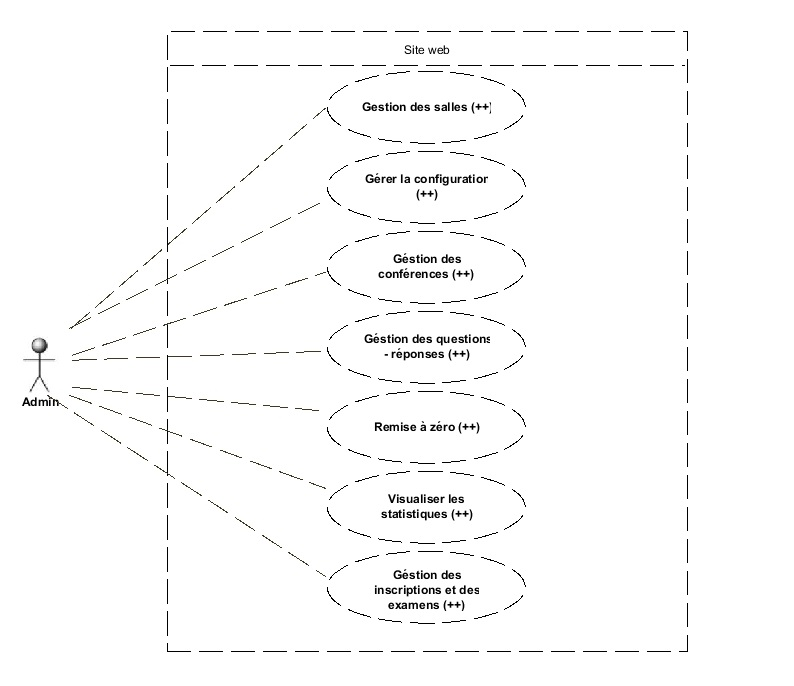
\includegraphics[scale=0.45]{images/Admin - menu1.jpg} 
        \end{center}
        \caption{Admin - menu}
        \label{Admin - menu}
    \end{figure}
\newpage

\item Il pourra par exemple s'occuper de la gestion des salles:
 \begin{figure}[h]
  \begin{center}
            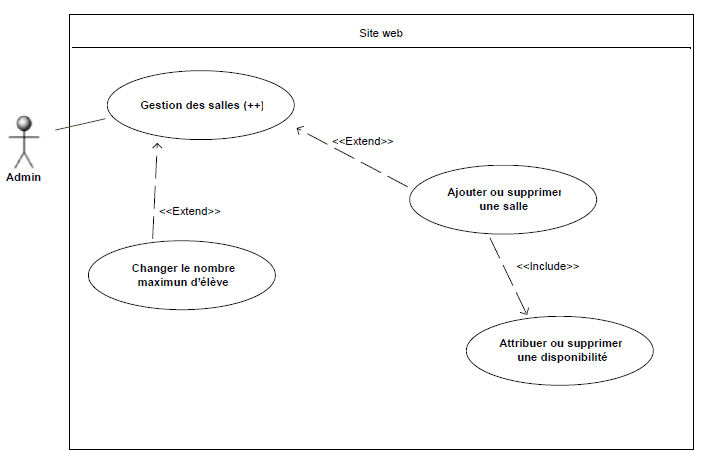
\includegraphics[scale=0.50]{images/Admin - salles.png} 
        \end{center}
        \caption{Admin - salles }
        \label{Admin - salles}
    \end{figure}
\end{itemize}
\newpage
 
    \section{Framework}

Pour la réalisation du site web, nous avions pensé organiser notre code en utilisant de simple scripts.
Ces pages utilisent l'architecture MVC (Modèle Vue contrôleur) afin de bien séparer chaque partie.

Chaque page aurait été accessible depuis l'index, et l'action fournie par l'url donne la page à afficher.
Ce développement ne convenait pas car la taille de l'application était un peu trop conséquente.

Nous avons donc appris davantage de techniques sur les patrons de conception, et avons organisé notre code
grâce à un framework "artisanal". Cette partie a pour but de présenter ce framework reposant sur l'architecture MVC.
Le framework récupère donc depuis l'url l'action du contrôleur et ses paramétres (optionnels) et exécute l'action.
Chaque action appartient donc à un module et existe en tant que route. Si une route est associée à une action existant dans
un module (i.e un contrôleur), alors elle est executée, et la page associée est générée puis envoyée.
Si la route n'existe pas, on est redirigé vers l'erreur 404 que nous avons défini.

        \subsection{L'architecture MVC}

Avant de décrire le framework que nous avons mis en place, une explication sur le patron de conception Modèle Vue contrôleur
est nécessaire. Il s'agit donc d'une architecture basée sur trois entités distinctes:

    \begin{itemize}
    \item Modèle
    \item Vue
    \item contrôleur
    \end{itemize}

Le modèle représente les données manipulées, principalement en accèdant en lecture et en écriture à la base de données.

La vue représente l'affichage, comment les informations sont agencées sur la page.

Le contrôleur représente la logique de l'application, c'est à dire le traitement des données obtenues par le modèle
qui sont destinées à être affichées par la vue.

L'élément central est donc le contrôleur, qui gère lui même pour chacune de ses actions son modèle et ses vues (plusieurs
manières d'afficher la même information).

        \subsection{Retour sur le framework}

La première classe, l'Application représente le pont entre tous ses composants. Il existe donc deux applications complémentaires, une pour les utilisateurs, et une pour les admins.
L'application contient les requêtes et les réponses HTTP, donnant ainsi les informations que l'utilisateur envoie et reçoit.

La classe HTTPRequest contient les variables GET et POST, les cookies ainsi que l'url entrée par l'utilisateur.
La classe HTTPResponse contient quant à elle la page associée à la réponse, et permet l'ajout de cookies, l'ajout d'entêtes
ainsi que l'exécution de la page, ou une redirection.

Les ApplicationComponants, constituent une partie de l'application, les blocs de base sur lequel repose le framework.
Chaque composant dispose d'une référence vers l'Application, ainsi, chaque composant est à même d'échanger avec les autres.
On retrouve bien la notion de pont pour l'Application.

La page elle même est composée d'un template et d'une vue générée.
Le template contient principalement le design général du site, le header, le menu ainsi que le footer.
La vue contient les informations relatives à la route choisie, c'est la partie la plus importante.

Une Page dérive également de l'ApplicationComponant, et permet donc de passer des variables depuis le contrôleur à la vue,
cette classe contient également le nom de la vue associée.

Il ne reste plus qu'à construire les contrôleurs de chaque module.
Afin de continuer avec l'approche orientée objet, on définit la classe BackController, qui permet d'être
suffisamment générique pour être commune à chaque futur contrôleur.

Le BackController contient donc les informations suivantes, obtenues depuis la route:

    \begin{itemize}
    \item Nom du module
    \item Nom de l'action
    \item Nom de la vue
    \item Référence vers la Page
    \end{itemize}

Chaque contrôleur est donc une classe dérivant du Backcontrôleur (qui lui même a accès aux autres portions de l'application).
Cela permet d'atteindre les autres parties du système et intéragir avec leurs utilisateurs.

Chaque action correspond à une méthode appartenant à la classe, et cette action est executée à l'appel de la page.
Le BackController se charge de récupérer la vue et de dire la Page de se générer. On peut ensuite utiliser HTTPResponse pour
renvoyer la Page à l'utilisateur.

Le modèle correspond aux données manipulées, et stockées en base de données. On accède en lecture et en écriture à la base de données
via des managers, qui permettent ainsi de manipuler la partie Modèle de l'architecture.

Les vues sont de simples fichiers PHP comprenant principalement du code XHTML. En effet, le but de ce fichier est de spécifier
l'affichage des informations du modèle, et manipulées dans le contrôleur. On y trouve un peu de scripting en PHP, surtout
pour y faire des affichages conditionnels, ainsi que des boucles pour afficher une séries d'informations liées.

Le User est une partie de l'application, il est donc dérivé de l'ApplicationComponant. Ici, le User identifie comme on peut
s'y attendre chaque utilisateur. L'utilisateur peut avoir ses propres attributs, et l'on détermine simplement s'il est authentifié
ou non. On peut associer un message flash (qui n'apparaît qu'une fois sur la page renvoyée à l'utilisateur), et qui est donc personnel
à l'utilisateur en cours.

Présenté un peu plus tôt, les managers sont essentiels pour manipuler les données de l'application. On crée donc une classe
Managers permettant d'exploiter la généricité sur chaque Manager spécifique que l'on va utiliser. Bien entendu, la classe
Managers dérive de l'ApplicationComponant afin d'être accessible principalement pour les contrôleurs spécifiques.

Chaque Manager manipule donc les classes "entités", ce sont juste une encapsulation de chaque information. Cela signifie
qu'un enregistrement dans la base de données correspond généralement à une instance d'une classe. Il y a bien entendu quelques
informations que nous ne stockons pas dans notre propre BDD (Base de données), mais que nous tirons de la BDD de Polytech.

Le Router est une classe qui dérive de l'ApplicationComponant, et qui récupère dans le contrôleur associé.
Une route s'écrit de la manière suivante:
<route url="/lectures/show-([0-9]+)\.html" module="lectures" action="show" vars="idPackage"/>
L'url du fichier contrôleur est indiquée, chaque contrôleur dispose d'un module associé, d'un nom d'action existant pour ce
contrôleur. On voit également qu'il est possible de fournir des valeurs dans l'url. Ces valeurs seront récupérées afin
d'être accessible en données GET. On peut mettre des conditions sur ces variables afin qu'elles respectent l'expression régulière
utilisée.

Nous utilisons également une fonctionnalité des serveurs apache, appelé URL-Rewritting. Cela consiste à ce que l'utilisateur
puisse entrer une certaine url, et que le serveur en reçoive une différente, qui sera donc traitée spécifiquement par le framework.
C'est ici que les routes interviennent, elles font le lien entre l'url de l'utilisateur et l'url donnée au serveur.

Le point fort de l'URL-Rewriting, et donc des routes, et de pouvoir assurer l'existence des pages liées au site web,
ainsi que de tester la validité des paramètres de la requête HTTP.

        \subsection{Classes annexes}

En plus du framework, nous avons créé quelques classes permettant de manipuler plus facilement, et de manière objet
des éléments revenant souvent dans le projet. En effet, nous utilisons de nombreuses fois des dates, et des horaires.

Nous avons donc une classe Date et une classe Time, permettant de créer des dates à partir de chaines de caractères,
on teste ainsi leur validité grâce à une expression régulière. On dispose également de primitives permettant de
faire des comparaisons entre des dates ou des heures. Le format est également adapté pour fonctionner avec MySQL.

Une classe permet également de générer automatiquement les formulaires utilisés, afin d'éviter au maximum les erreurs,
et de simplifier la lecture des vues.

// class Database William

        \cite{ref_framework_mvc}

    \section{style graphique}
Le fonctionnement du site est une chose importante, mais l'utilisateur n'est ne voit pas comment cela fonctionne. 
Il ne voit que le site web à travers le style qu'on lui aura appliqué. Il est dons important de faire en sorte que le site
soit plaisant aux yeux du l'utilisateur. Nous avons opté pour une dominante bleu, 
rapellant les couleurs de Polytech, nuancée par une touche de blanc.
  \begin{figure}[h]
        \begin{center}
        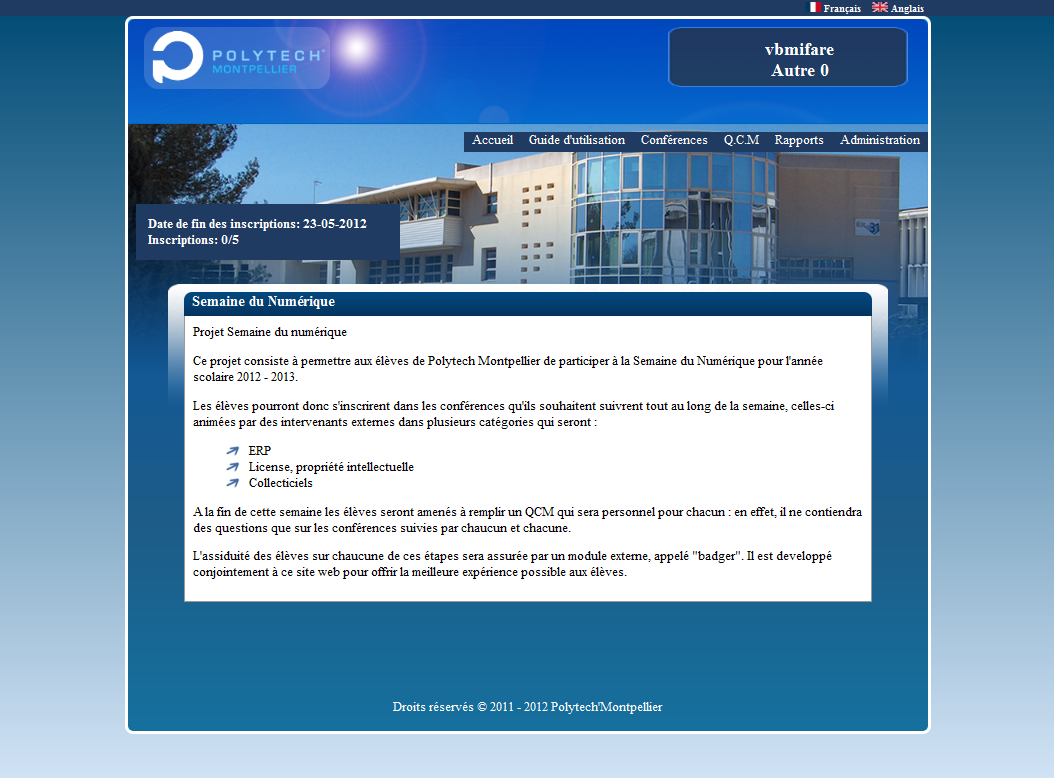
\includegraphics[scale=0.4]{images/screenSiteWeb.png} 
        \end{center}
        \caption{Site web}
        \label{Site web}
     \end{figure} 

    \section{Règles d'utilisation}

        \subsection{Check list}



        \subsection{Recommandations}


